\begin{fact} \label{iso-rect}
	Considérons tous les rectangles de périmètre fixé $p$. Parmi tous ces rectangles, celui d'aire maximale est le carré de côté $c = \num{.25} p$.
\end{fact}


\begin{proof}
	Une preuve courante est d'exprimer l'aire du rectangle comme un polynôme du 2\ieme\ degré en $L$ par exemple.%
	\footnote{
		L'aire est donnée par $L \ell = L (\num{.5} p - L)$ qui est maximale en $L_M = \num{.25} p$ (moyenne des racines), d'où $\ell_M = \num{.25} p = L_M$.
	}
	On peut en fait faire plus simplement grâce au dessin suivant où les rectangles $1$, $2$ et $3$ sont isométriques au rectangle vert étudié de dimension $L \times \ell$.

	\begin{center}
		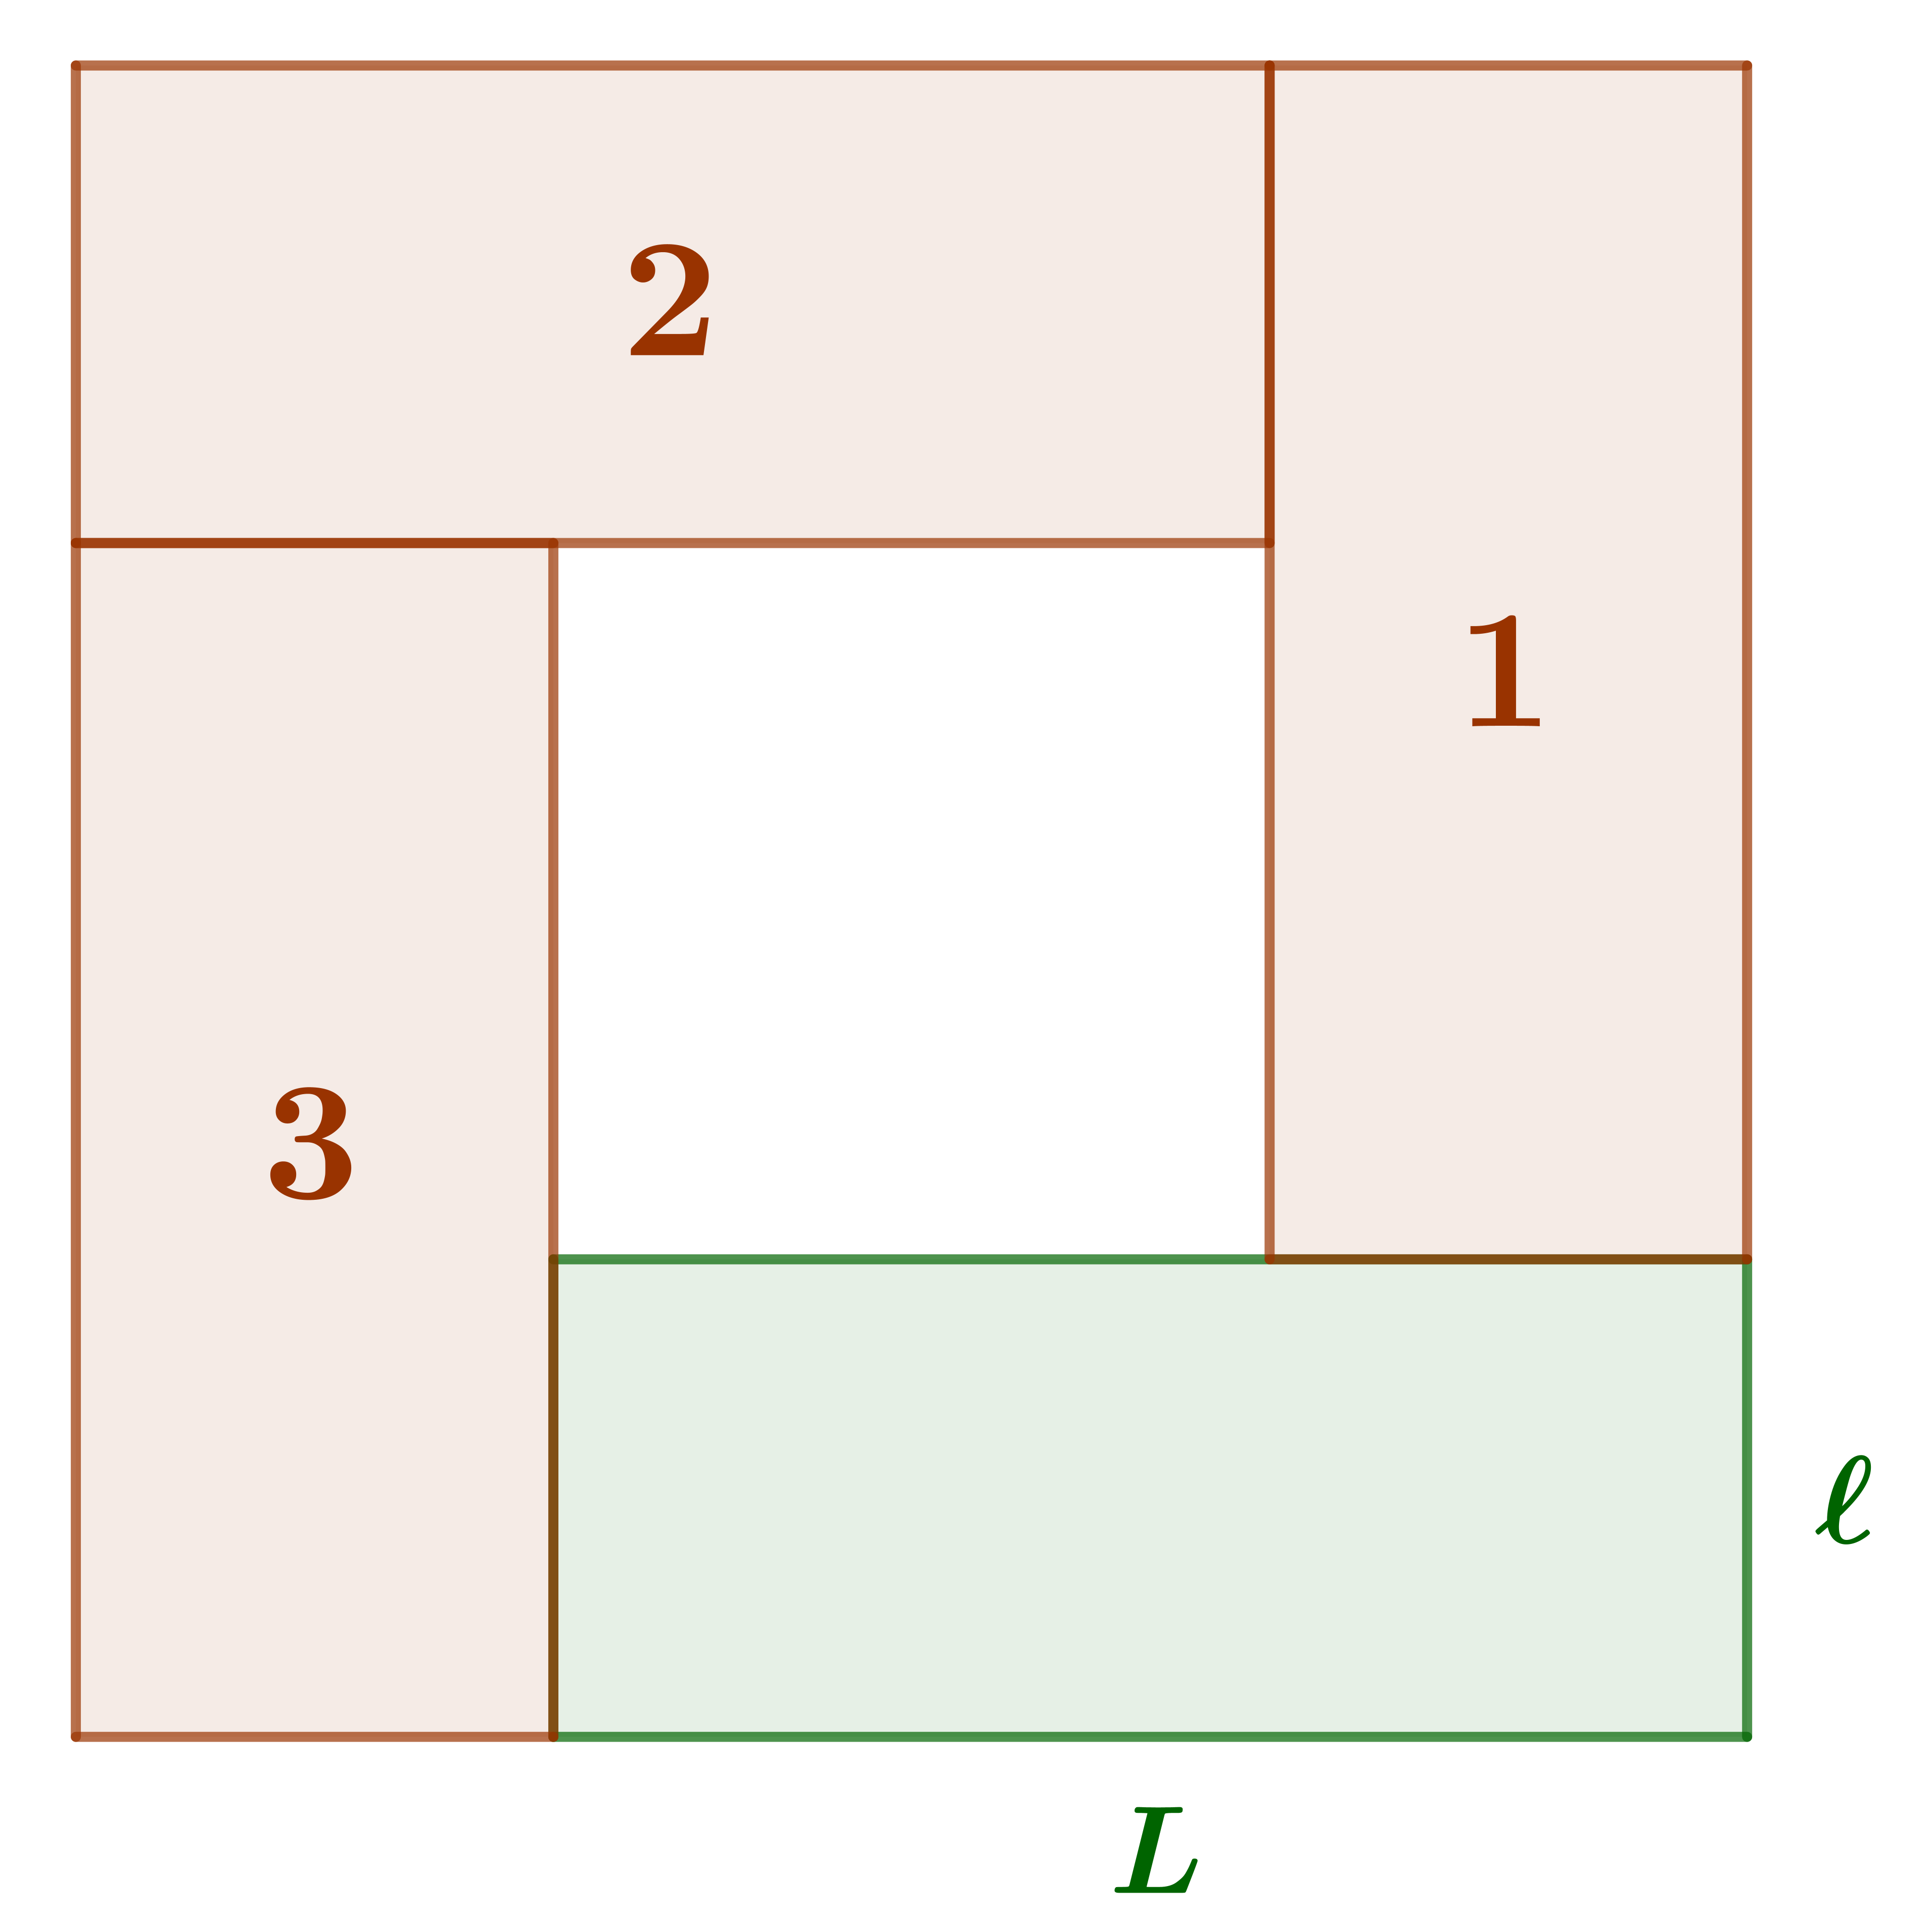
\includegraphics[scale=.4]{content/rectangle/rectangle.png}
	\end{center}
	
	Le raisonnement tient alors aux constations suivantes accessibles à un collégien.
	%
	\begin{enumerate}
		\item Le grand carré a un aire supérieure ou égale à $4 L \ell$.

		\item Le grand carré a un périmètre égal à $4 (L + \ell)$.

		\item Via une homothétie de rapport \num{.5}\,, nous obtenons un carré d'aire supérieure ou égale à $\num{.5}^2 \times 4 L \ell =  L \ell$, et de périmètre égal à $\num{.5} \times 4 (L + \ell) = 2 (L + \ell)$.
	\end{enumerate}
	
	Donc pour tout rectangle de périmètre $p = 2 (L + \ell)$ et d'aire $\mathscr{A} = L \ell$, nous pouvons construire un carré de périmètre identique, mais avec une aire supérieure ou égale à $\mathscr{A}$. Joli! Non?
\end{proof}


\begin{remark}
	Au passage, nous avons pour $(L ; \ell) \in \big( \RRsp \big)^2$, $4 L \ell \leq (L + \ell)^2$, c'est-à-dire $2 L \ell \leq L^2 + \ell^2$, d'où $\sqrt{L \ell} \leq \sqrt{\dfrac12 (L^2 + \ell^2)}$, soit la comparaison des moyennes géométriques et quadratiques d'ordre $2$.
\end{remark}
